\chapter{Learning to Trade Power}
\label{ch:learningtotrade}
This chapter examines the convergence to a Nash equilibrium of agents
compteting with portfolios of generating plant.  Value function based and
policy gradient reinforcement learning algorithms are compared in their speed
of convergence and sensitivity to parameter changes using a six bus electric
power system model.

\section{Introduction}
To the best of the author's knowledge, this thesis presents the first case of
policy gradient reinforcement learning methods being applied to electricity
trading problems.  As a first step it is necessary to confirm that when using
these methods, a system of multiple agents will converge to the same Nash
equilibrium that conventional closed-form simulation techniques produce.

This is the same approach by \citeA{krause:nash06} before performing the study
of congestion management techniques that is reviewed in Section
\ref{sec:related_cong}.  Informally, a Nash equlibrium is a point at which no
player is motivated to deviate from its strategy.  This can be difficult
to determine in complex systems so the experiment presented here utilises a
model simple enough that it can be determined through exhaustive search.

By observing the actions taken and the reward received by each agent over the
initial simulation periods it is possible to compare different configurations
of the algorithms in their speed of convergence to an optimal policy.  In the
following sections the objectives of this experiment are explictly defined, the
setup of the simulations is explained and simulation results are provided with
discussion and critical analysis.

\section{Aims and Objectives}
Some elements of this experiment are very similar to those presented in
\citeA{krause:nash06} and one aim is to reproduce those results.  Additionally,
the specific objectives are to show that:
\begin{itemize}
  \item Policy gradient methods converge to the same Nash equilibrium as value
  function based methods.
  \item The differences in speed of convergence to an optimal policy between
  the learning methods.
  \item The sensitivity of policy convergence to algorithm parameter choices
  and policy function approximation structure.
\end{itemize}
Meeting these objectives aims to provide a basis for more complicated
experiments that are less intuitively tractable.

\section{Method of Simulation}
% Each learning method is tested individually using a range of parameter
% configurations.  A power system model with one bus, one generator $k$ and
% one dispatchable load $l$.  In this
% context, the market clearing process is equivalent to creating offer and bids
% stacks and finding the point of intersection.  A passive agent is associated
% with the dispatchable load.  This agent bids for $-p_{g,l}^{min}$ at marginal
% cost each period regardless of environment state or reward signal.  A
% dispathcable load is used instead of a constant load to allow a price to be
% set. Generator $k$ is given sufficient capacity to supply the demand
% of the dispatchable load, $p_{g,k}^{max} > -p_{g,l}^{min}$, and the marginal of
% the $k$ is half that of the load $l$.  The generator and dispatchable load
% attributes are given in Table X.  A price cap for the market is set to twice the
% marginal cost of the $l$ at full capacity, $p_{g,l}^{min}$.  The DC optimal
% power flow formulation (See Section \ref{sec:opf}, above) is used to clear the
% market and reactive power trade is omitted.
Learning methods are compared in this experiment by repeating the same
simulation with the different algorithms in-place.  An alternative
might be to use a combination of methods in the same simulation, but the
approach used here is intended to be an extension of the work in
\citeA{krause:nash06}.

Each simulation uses the 6-bus electric power system model from \citeA[pp.~104,
112, 119, 123-124, 549]{wood:pgoc}.  The six buses in this model are at 230kV
and are connected by eleven transmission lines.  It contains three generating
units with a total capacity of 530MW and loads at three locations, each of
70MW. The generator opertaing costs are linear functions of production, defined by
the parameters in Table \ref{tbl:case6ww_gencost} and plotted in Figure X.
The connectivity of the branches and the locations of the generators and the
load is shown in Figure~\ref{fig:case6ww}.  Data for the power system model is
provided in Appendix \ref{adx:case6ww} and is distributed with the software
developed for this thesis (See Appendix \ref{sec:pylon}).

%\begin{figure}
\label{fig:case6ww}
\centering
\begin{scriptsize}
\begin{tikzpicture}[thick]

\coordinate (c1) at (0,4);
\coordinate (c2) at (5,6.5);
\coordinate (c3) at (10,4);
\coordinate (c4) at (0,0);
\coordinate (c5) at (5,-2.5);
\coordinate (c6) at (10,0);
\coordinate (over) at (0,3.75);

\busbar{b1}{c1}{20mm}
\busbar{b2}{c2}{30mm}
\busbar{b3}{c3}{20mm}
\busbar{b4}{c4}{20mm}
\busbar{b5}{c5}{30mm}
\busbar{b6}{c6}{20mm}

% Branch 1-2.
\draw[line] ([xshift=5mm] b1.north) node[rotate=90,above right]{$15.41$}
node[rotate=90,below right]{$-9.58$} -- ++(0,3.75) -| ([xshift=-8mm] b2.north)
node[rotate=90,above right]{$-15.14$} node[rotate=90,below right]{$5.70$};
% Branch 1-4.
\draw[line] ([xshift=-5mm] b1.south) node[rotate=90,above left]{$33.95$}
node[rotate=90,below left]{$22.50$} -- ([xshift=-5mm] b4.north)
node[rotate=90,above right]{$-33.15$} node[rotate=90,below right]{$-23.46$};
% Branch 1-5.
\draw[line] ([xshift=5mm] b1.south) node[rotate=90,above left]{$27.86$}
node[rotate=90,below left]{$12.80$} -- ([xshift=5mm,yshift=-15mm] b1.south)
-- ([xshift=-8mm,yshift=15mm] b5.north) -- ([xshift=-8mm] b5.north)
node[rotate=90,above right]{$-27.11$} node[rotate=90,below right]{$-16.20$};
% Branch 2-3.
\draw[line] ([xshift=8mm] b2.north) node[rotate=90,above right]{$0.29$}
node[rotate=90,below right]{$-11.76$} -- ++(0,1.25) -| ([xshift=-5mm] b3.north)
node[rotate=90,above right]{$-0.25$} node[rotate=90,below right]{$5.18$};
% Branch 2-4.
\draw[line,ultra thick] ([xshift=-8mm] b2.south) node[rotate=90,above
left]{$41.74$} node[rotate=90,below left]{$43.11$} --
([xshift=-8mm,yshift=-15mm] b2.south) -- node[sloped,above]{$\vert S_{max}^5
\vert = 60.0$} ([xshift=5mm,yshift=15mm] b4.north) -- ([xshift=5mm] b4.north)
node[rotate=90,above right]{$-40.06$} node[rotate=90,below right]{$-41.83$};
% Branch 2-5.
\draw[line] (b2.south) node[rotate=90,above left]{$17.35$}
node[rotate=90,below left]{$14.93$} -- (b5.north) node[rotate=90,above
right]{$-16.81$} node[rotate=90,below right]{$-17.46$};
% Branch 2-6.
\draw[line] ([xshift=8mm] b2.south) node[rotate=90,above left]{$25.03$}
node[rotate=90,below left]{$12.67$} -- ([xshift=8mm,yshift=-15mm] b2.south)
-- ([xshift=-5mm,yshift=15mm] b6.north) -- ([xshift=-5mm] b6.north)
node[rotate=90,above right]{$-24.49$} node[rotate=90,below right]{$-16.38$};
% Branch 3-5.
\draw[line] ([xshift=-5mm] b3.south) node[rotate=90,above left]{$23.18$}
node[rotate=90,below left]{$21.57$} -- ([xshift=-5mm,yshift=-15mm] b3.south)
-- ([xshift=8mm,yshift=15mm] b5.north) -- ([xshift=8mm] b5.north)
node[rotate=90,above right]{$-21.99$} node[rotate=90,below right]{$-24.28$};
% Branch 3-6.
\draw[line] ([xshift=5mm] b3.south) node[rotate=90,above left]{$47.50$}
node[rotate=90,below left]{$59.90$} -- ([xshift=5mm] b6.north)
node[rotate=90,above right]{$-46.45$} node[rotate=90,below right]{$-56.82$};
% Branch 4-5.
\draw[line] ([xshift=5mm] b4.south) node[rotate=90,above left]{$3.21$}
node[rotate=90,below left]{$-4.71$} -- ++(0,-3.75) -| ([xshift=-8mm] b5.south)
node[rotate=90,above left]{$-3.19$} node[rotate=90,below left]{$-3.03$};
% Branch 5-6.
\draw[line] ([xshift=8mm] b5.south) node[rotate=90,above left]{$-0.90$}
node[rotate=90,below left]{$-9.03$} -- ++(0,-1.25) -| ([xshift=-5mm] b6.south)
node[rotate=90,above left]{$0.94$} node[rotate=90,below left]{$3.21$};

% Generator 1.
\genset{g1}{$(c1)+(-5mm,15mm)$}
\draw[line] ([xshift=-5mm] b1.north) -- node[sloped,above]{$77.22$}
node[sloped,below]{$25.72$} (g1.south);
% Generator 2.
\genset{g2}{$(c2)+(0,15mm)$}
\draw[line] (b2.north) -- node[sloped,above]{$69.27$}
node[sloped,below]{$64.65$} (g2.south);
% Generator 3.
\genset{g3}{$(c3)+(5mm,15mm)$}
\draw[line] ([xshift=5mm] b3.north) -- node[sloped,above]{$70.42$}
node[sloped,below]{$86.64$} (g3.south);

% Load 1.
\loadd{l1}{$(c4)-(5mm,15mm)$}
\draw[line] (l1.south) -- node[sloped,above]{$70.00$}
node[sloped,below]{$70.00$} ([xshift=-5mm] b4.south);
% Load 2.
\loadd{l2}{$(c5)-(0mm,15mm)$}
\draw[line] (l2.south) -- node[sloped,above]{$70.00$}
node[sloped,below]{$70.00$} (b5.south);
% Load 3.
\loadd{l3}{$(c6)+(5mm,-15mm)$}
\draw[line] (l3.south) -- node[sloped,above]{$70.00$}
node[sloped,below]{$70.00$} ([xshift=5mm] b6.south);

\end{tikzpicture}
\end{scriptsize}
\caption{One line diagram for six bus power system model from [].}
\end{figure}


No load profile is defined, the system load is assumed to be peak for all
simulation periods, so only one system state is defined for the value function
based algorithms.  The minimum operating point, $P^{min}$, for all generators
is made to be zero so as to simplify the experiment and avoid the need to
use the unit decommitment algorithm defined in Section \ref{sec:decommit}.

Two active agents, and one passive agent that always offers at marginal cost,
are defined in each simulation and are each associated with one generating
unit. Their activity in the market is restricted to one offer of maximum
capacity in each period, at a price representing a markup of between 0 and 30\%
on marginal cost.  Value function based methods are restricted to discrete markup steps of
10\%, giving possible markup actions of 0, 10, 20 and 30\%, as illustrated in
Figure X.  The market price cap is set such that it is never reached by any
markup and does not complicate the experiment.

The learning methods compared are Sarsa, Q-learning, Q($\lambda$), ENAC,
REINFORCE and the variant Roth-Erev technique.  The parameters available to
adjustment are\ldots.

As in \citeA{krause:nash06}, the point of Nash equilibrium is established by
computing each agent's reward for all possible combinations of markup.  The
value are given in Table Y.

As one would intuitively expect, the optimal policy for each agent is to apply
the maximum markup to each offer as this never results in a generator failing
to be dispatched.

They show that the optimal point is where the agent with the lowest cost
generator applies the maximum markup and the agent with the medimum priced
generator offers a proce just below the marginal cost of the passive
agent's generator.


\section{Results}

\begin{figure}
  \centering
  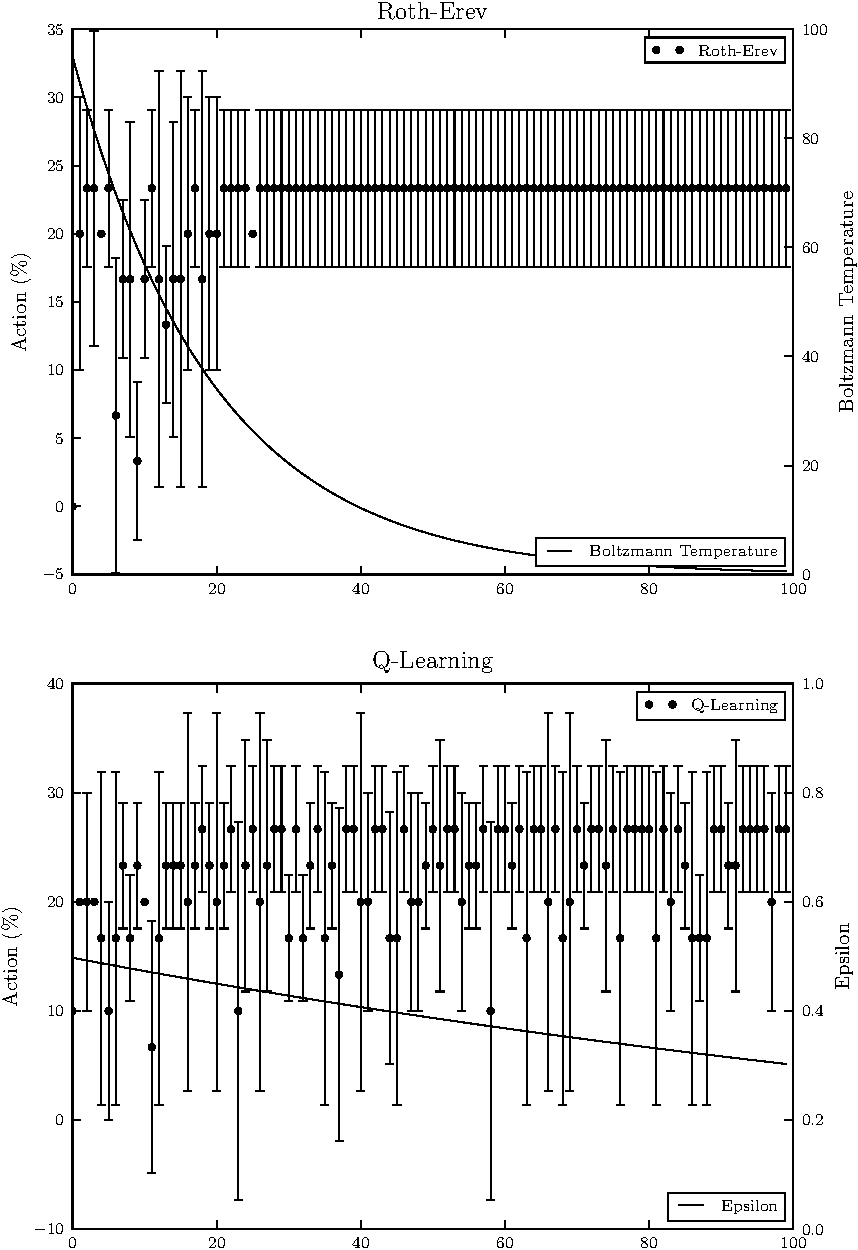
\includegraphics{figures/fig5_1_g1_action}
  \caption{Average markup for agent 1 and standard deviation over 10 runs.}
  \label{fig:libpsat}
\end{figure}

\section{Discussion}
\section{Conclusions}


% \chapter{Competitive Power Trade}
% Having compared the learning methods in a one-player context, this section
% describes the method used to pit them against one and other and compare their
% performance.
%
% \section{Aims \& Objectives}
% Competition is fundamental to markets and this experiment aims to compare
% learning methods in a complex dynamic market environment with multiple
% competing participants.  The objective is to compare:
% \begin{itemize}
%   \item Performance, in terms of profitability, over a finite number of
%   periods,
%   \item Profitability when trading both active and reactive power.
%   \item Consistency of profit making and,
%   \item Sensitivity to algorithm parameter changes.
% \end{itemize}
%
% \section{Method of Simulation}
% Figure X illustrates the structure of the six bus power system model, from
% \cite{wood:pgoc}, with three generators and fixed demand at three of the buses
% used to provide a dynamic environment with typical system values.  Bus,
% branch and generator attribute values are stated in Tables X, Y, Z,
% respectively.  Three learning methods are compared in six simulations
% encapsulating all method--generator combinations.
%
% A price cap $c_{cap}$ of twice the marginal cost of the most expensive generator
% at full capacity is set by the market.  The simulations are repeated for with agents
% actions composing both price and quantity and with just price.  For the
% value-function methods, the state is defined by the market clearing price from
% the previous period, divided equally into $x_s$ discrete states between $0$ and
% $c_{cap}$.  The state vector $s_t$ for the policy gradient methods consists of
% the market clearing price and generator set-point from the previous period.
% \begin{equation}
% s_t =
% \begin{bmatrix}
% c_{mcp}\\
% p_g
% \end{bmatrix}
% \end{equation}
% The script used to conduct the simulation is provided in Listing X.

\chapter{System Constraint Exploitation}
\label{ch:exploitation}
% One of the main features of agents using policy gradient learning methods and
% artifical neural networks for policy function approximation is their ability to
% accept many signals of continuous sensor data.  This section describes an
% experiment in which the power system is severly constrained for certain
% periods, resulting in elevated nodal marginal prices in particular areas.  The
% methods are tested in their ability to exploit these constraints and improve
% their total accumulated reward.
This chapter explores the exploitation of constraints in electric power
system models by agents whose behaviour is determined by reinforcement learning
algorithms.  Value function based and policy gradient methods are compared
using the IEEE Reliability Test System, with dynamic loads and probabilistic
transmission line outages.

\section{Introduction}
Having explored the basic properties of various learning methods in
Chapter~\ref{ch:learningtotrade}, this experiment examines them under a complex dynamic scenario.  Policy gradient methods have been used in robotic control
applications with multi-dimensional, continuous state and action spaces, and
exhibit a degree of robustness to sensor noise.  In this experiment,
these features are explored in the context of learning to trade power.

Control of a portfolio of generators using continous sensor data from
simulations of a standard test power system model with realisitic load dynamics
is examined.  To force the system into a constrained state at certain times, transmission line outages are simualated according to the probabilities given in Table Z.  By
observing the actions taken and the reward received by an agent during these
periods it is examined if these methods can be used to exploit such
occurances.

\section{Aims and Objectives}
This experiment aims to compare the operation of learning methods in dynamic
electric power system environments.  Specifically, the objective are to
determine:
\begin{itemize}
  \item If policy gradient methods can be used to achieve greater profit under
  dynamic loading conditions.
  \item If policy gradient methods can exploit outages and the resulting system
  constraints to further increased profit.
  \item The value of using AC optimal power flow formulations in agent base
  electricity market simulation.
\end{itemize}
Meeting these objectives aims to demonstrate the value of policy gradient
methods in electricity market participant modelling.

\section{Method}
The learning methods are compared by repeating the same simulation with
different types of algorithm in-place.  Some simplification of the state
and action domains for the value function based methods is required, but the
portfolios of generation and load profiles are constant.

The IEEE Reliability Test System \cite{ieee79rts} provides the power system
model, load profiles and outage probabilities used in each simulation.  The
model has 24 bus locations, connected by 32 transmission lines, 4 transformers
and 2 underground cables.  The transformers tie together two system areas at
230kV and 138kV.  The model has 32 generators of 9 different types (See Table
X) with a total capacity of 3.45GW and load at 17 locations, totalling 2.85GW.
Generator costs are quadratic functions of output, defined by the parameters in
Table Y.  Figure X plots the cost functions for each type of generator over
their production range and illustrates their categorisation by fuel type.  Data
for the model is provided in Appendix \ref{adx:ieee_rts} and the connectivity
of branches and the location of generators and loads is illustrated in
Figure~Y.

The generating stock is divided into 5 portfolios, as listed in Table Z, that
are each endowed to a learning agent.  The synchronous generator is associated
with a passive agent that always offers at marginal cost i.e.~\$/MWh~0.
Markups of offer price are restricted a maximum of 30\% and discrete markup
steps of 10\% are defined for value function based methods.

%\newcommand{\generatorunit}[3]{
  \node[circle,draw,thick,minimum width=6mm,#3] (#1) at (#2) {};
  \draw[thick] ($(#2)-(2mm,0)$) sin ++(1mm,1mm) cos ++(1mm,-1mm)
  sin ++(1mm,-1mm) cos ++(1mm,1mm);
}

\begin{figure}
\centering
\small
\begin{tikzpicture}[thick,label distance=0mm]
  \tikzstyle{busbar} = [rectangle,draw,fill=black!50,inner sep=0pt];
  \tikzstyle{hbus} = [busbar,minimum width=10mm,minimum height=2pt];
  \tikzstyle{vbus} = [busbar,minimum width=2pt,minimum height=10mm];
  \tikzstyle{overhead} = [-,thick];
  \tikzstyle{cable} = [thick];
  \tikzstyle{trxcircle} = [circle,draw=black,inner sep=0pt,minimum width=5mm];
  \tikzstyle{every pin edge}=[-,shorten <=1pt,thin];

\node[hbus,minimum width=15mm,label=left:Bus 1] (bus1) at (5,0) {};
\node[hbus,minimum width=15mm,label=right:Bus 2] (bus2) at (7,0) {};
\node[hbus,label=right:Bus 3] (bus3) at (0,6) {};
\node[vbus,label=above:Bus 4] (bus4) at (3,4) {};
\node[vbus,label=above:Bus 5] (bus5) at (6.5,3) {};
\node[vbus,label=above:Bus 6] (bus6) at (12,5.3) {};
\node[hbus,label=right:Bus 7] (bus7) at (11,0.5) {};
\node[vbus,label=above:Bus 8] (bus8) at (12,3) {};
\node[hbus,minimum width=20mm,label=left:Bus 9] (bus9) at (5,6) {};
\node[hbus,minimum width=20mm,label=right:Bus 10] (bus10) at (8,6) {};
\node[hbus,minimum width=20mm,label=left:Bus 11] (bus11) at (5,8) {};
\node[hbus,minimum width=20mm,label=right:Bus 12] (bus12) at (8,8) {};
\node[vbus,label={[xshift=-4mm]below:Bus 13}] (bus13) at (12,10) {};
\node[vbus,label=above:Bus 14] (bus14) at (3.5,11.5) {};
\node[hbus,minimum width=20mm,label=right:Bus 15] (bus15) at (0.5,12) {};
\node[hbus,minimum width=15mm,label=right:Bus 16] (bus16) at (0,14) {};
\node[vbus,minimum height=20mm,label=above:Bus 17] (bus17) at (-1,16) {};
\node[hbus,minimum width=20mm,label=right:Bus 18] (bus18) at (2,18) {};
\node[hbus,label=below right:Bus 19] (bus19) at (4.5,14) {};
\node[hbus,minimum width=15mm,label=below right:Bus 20] (bus20) at (7,14) {};
\node[hbus,minimum width=25mm,label=right:Bus 21] (bus21) at (5,17) {};
\node[hbus,label=right:Bus 22] (bus22) at (9,17) {};
\node[vbus,minimum height=15mm,label=above:Bus 23] (bus23) at (11,14.55) {};
\node[hbus,label=right:Bus 24] (bus24) at (0,8) {};

% Branch 1-2.
\draw[cable] ([xshift=5mm] bus1.north) -- ++(0,5mm) node[xshift=5mm,above]
{cable} -| ([xshift=-5mm] bus2.north);
% Branch 1-3.
\draw[overhead] ([xshift=-5mm] bus1.north) -- ([xshift=-5mm,yshift=5mm]
bus1.north) -- ([xshift=0mm,yshift=-5mm] bus3.south) -- (bus3.south);
% Branch 1-5.
\draw[overhead] (bus1.north) |- (bus5.west);
% Branch 2-4.
\draw[overhead] (bus2.north) -- ([yshift=5mm] bus2.north) -- ([xshift=5mm]
bus4.east) -- (bus4.east);
% Branch 2-6.
\draw[overhead] ([xshift=5mm] bus2.north) -- ([xshift=5mm,yshift=5mm]
bus2.north) -- ([xshift=-5mm,yshift=-3mm] bus6.west) -- ([yshift=-3mm]
bus6.west);
% Branche 3-9.
\draw[overhead] ([xshift=3mm] bus3.south) -- ++(0,-5mm) -| ([xshift=-5mm]
bus9.south);
% Branch 3-24.
\draw node[trxcircle,yshift=-1mm,above of=bus3] (t3-24p) {};
\draw node[trxcircle,yshift=1mm,above of=bus3] (t3-24s) {};
\draw[overhead] (bus3.north) -- (t3-24p.south);
\draw[overhead] (t3-24s.north) -- (bus24.south);
% Branch 4-9.
\draw[overhead] ([yshift=3mm] bus4.east) -- ([xshift=5mm,yshift=3mm] bus4.east)
-- ([yshift=-5mm] bus9.south) -- (bus9.south);
% Branch 5-10.
\draw[overhead] (bus5.east) -| (bus10.south);
% Branch 6-10.
\draw[overhead] (bus6.west) -| node[above right] {cable} ([xshift=5mm]
bus10.south);
% Branch 7-8.
\draw[overhead] ([xshift=-3mm] bus7.north) |- ([yshift=-3mm] bus8.west);
% Branch 8-9.
\draw[overhead] (bus8.west) -- ([xshift=-5mm] bus8.west) --
([xshift=5mm,yshift=-5mm] bus9.south) -- ([xshift=5mm] bus9.south);
% Branch 8-10;
\draw[overhead] ([yshift=3mm] bus8.west) -- ([xshift=-5mm,yshift=3mm]
bus8.west) -- ([xshift=-5mm,yshift=-10mm] bus10.south) -- ([xshift=-5mm]
bus10.south);
% Branch 9-11.
\draw node[trxcircle,yshift=-1mm,xshift=-5mm,above of=bus9] (t9-11p) {};
\draw node[trxcircle,yshift=1mm,xshift=-5mm,above of=bus9] (t9-11s) {};
\draw[overhead] ([xshift=-5mm] bus9.north) -- (t9-11p.south);
\draw[overhead] (t9-11s.north) -- ([xshift=-5mm] bus11.south);
% Branch 9-12.
\draw node[trxcircle,yshift=-1mm,xshift=-5mm,node distance=7mm,below of=bus12]
(t9-12p) {};
\draw node[trxcircle,yshift=1mm,xshift=-5mm,node distance=7mm,below of=bus12]
(t9-12s) {};
\draw[overhead] ([xshift=5mm] bus9.north) -- ([xshift=5mm,yshift=3mm]
bus9.north) -- ([yshift=-3mm] t9-12p.south) -- (t9-12p.south);
\draw[overhead] (t9-12s.north) -- ([xshift=-5mm] bus12.south);
% Branch 10-11.
\draw node[trxcircle,yshift=-1mm,xshift=5mm,node distance=7mm,below of=bus11]
(t10-11p) {};
\draw node[trxcircle,yshift=1mm,xshift=5mm,node distance=7mm,below of=bus11]
(t10-11s) {};
\draw[overhead] ([xshift=-5mm] bus10.north) -- ([xshift=-5mm,yshift=3mm]
bus10.north) -- ([yshift=-3mm] t10-11p.south) -- (t10-11p.south);
\draw[overhead] (t10-11s.north) -- ([xshift=5mm] bus11.south);
% Branch 10-12.
\draw node[trxcircle,yshift=-1mm,xshift=5mm,above of=bus10] (t10-12p) {};
\draw node[trxcircle,yshift=1mm,xshift=5mm,above of=bus10] (t10-12s) {};
\draw[overhead] ([xshift=5mm] bus10.north) -- (t10-12p.south);
\draw[overhead] (t10-12s.north) -- ([xshift=5mm] bus12.south);
% Branch 11-13.
\draw[overhead] ([xshift=5mm] bus11.north) -- ([xshift=5mm,yshift=5mm]
bus11.north) -- ([xshift=-5mm] bus13.west) -- (bus13.west);
% Branch 11-14.
\draw[overhead] ([xshift=-5mm] bus11.north) |- ([yshift=-3mm] bus14.east);
% Branch 12-13.
\draw[overhead] ([xshift=-5mm] bus12.north) -- ([xshift=-5mm,yshift=7mm]
bus12.north) -- ([xshift=-5mm,yshift=-3mm] bus13.west) -- ([yshift=-3mm]
bus13.west);
% Branch 12-23.
\draw[overhead] ([xshift=5mm] bus12.north) |- ([yshift=-5mm] bus23.west);
% Branch 13-23.
\draw[overhead] ([yshift=3mm] bus13.west) -- ([xshift=-5mm,yshift=3mm]
bus13.west) |- ([yshift=-5mm] bus23.east);
% Branch 14-16.
\draw[overhead] ([yshift=3mm] bus14.west) -- ([xshift=-6mm,yshift=3mm]
bus14.west) |- ([xshift=5mm,yshift=-5mm] bus16.south) -- ([xshift=5mm]
bus16.south);
% Branch 15-16.
\draw[overhead] ([xshift=-5mm] bus15.north) -- (bus16.south);
% Branches 15-21.
\draw[overhead] (bus15.north) -- ([yshift=5mm] bus15.north) -- ([yshift=-10mm]
bus21.south) -- (bus21.south);
\draw[overhead] ([xshift=5mm] bus15.north) -- ([xshift=5mm,yshift=5mm]
bus15.north) -- ([xshift=5mm,yshift=-10mm] bus21.south) -- ([xshift=5mm]
bus21.south);
% Branch 15-24.
\draw[overhead] ([xshift=-5mm] bus15.south) -- (bus24.north);
% Branch 16-17.
\draw[overhead] ([xshift=-5mm] bus16.north) |- ([yshift=-5mm] bus17.east);
% Branch16-19.
\draw[overhead] ([xshift=5mm] bus16.north) -- ([xshift=5mm,yshift=5mm]
bus16.north) -| ([xshift=-3mm] bus19.north);
% Branch 17-18.
\draw[overhead] ([yshift=5mm] bus17.east) -| ([xshift=-5mm] bus18.south);
% Branch 17-22.
\draw[overhead] (bus17.east) -- ([xshift=20mm] bus17.east) -- ([xshift=20mm,
yshift=-5mm] bus17.east) -| ([xshift=3mm] bus22.south);
% Branches 18-21.
\draw[overhead] (bus18.south) -- ([yshift=-20mm] bus18.south) -|
([xshift=-5mm] bus21.south);
\draw[overhead] ([xshift=5mm] bus18.south) -- ([xshift=5mm,yshift=-15mm]
bus18.south) -| ([xshift=-10mm] bus21.south);
% Branches 19-20.
\draw[overhead] (bus19.north) -- ([yshift=10mm] bus19.north) -|
([xshift=-1.5mm] bus20.north);
\draw[overhead] ([xshift=3mm] bus19.north) -- ([xshift=3mm,yshift=5mm]
bus19.north) -| ([xshift=-4.5mm] bus20.north);
% Branches 20-23.
\draw[overhead] ([xshift=1.5mm] bus20.north) |- ([yshift=5mm] bus23.west);
\draw[overhead] ([xshift=4.5mm] bus20.north) |- (bus23.west);
% Branch 21-22.
\draw[overhead] ([xshift=10mm] bus21.south) -- ([xshift=10mm,yshift=-7.5mm]
bus21.south) -| ([xshift=-3mm] bus22.south);

% Generator @ Bus 1.
\generatorunit{gen1}{4.5,-0.8}{label=left:192 MW,pin={[pin distance=12mm,text
centered,text width=10.5mm]165:2$\times$U20 2$\times$U76}};
\draw[overhead] ([xshift=-5mm] bus1.south) -- (gen1.north);
% Generator @ Bus 2.
\generatorunit{gen2}{7.5,-0.8}{label=right:192 MW,pin={[pin distance=12mm,text
centered,text width=10.5mm]15:2$\times$U20 2$\times$U76}};
\draw[overhead] ([xshift=5mm] bus2.south) -- (gen2.north);
% Generator @ Bus 7.
\generatorunit{gen3}{11,-0.3}{label=right:300 MW,pin=below:3$\times$U100};
\draw[overhead] (bus7.south) -- (gen3.north);
% Generator @ Bus 13.
\generatorunit{gen4}{12.3,10.9}{label=above:591 MW,pin={[pin distance=8mm]
left:3$\times$U197}};
\draw[overhead] ([yshift=3mm] bus13.east) -- ([yshift=3mm,xshift=2.5mm]
bus13.east) -- (gen4.south);
% Generator @ Bus 14.
\generatorunit{gen5}{4.3,11.8}{label={[text justified,text
width=15mm]right:Synch. Cond.}}; \draw[overhead] ([yshift=3mm] bus14.east) --
(gen5.west);
% Generator @ Bus 15.
\generatorunit{gen6}{0.5,11.2}{label={[text centered,text width=10mm]below:215 MW},
pin={[pin distance=5mm,text centered,text width=15mm]-70:5$\times$U12
1$\times$U155}}; \draw[overhead] (bus15.south) -- (gen6.north);
% Generator @ Bus 16.
\generatorunit{gen7}{0.0,15}{label=right:155 MW};
\draw[overhead] (bus16.north) -- (gen7.south);
% Generator @ Bus 18.
\generatorunit{gen8}{1.5,18.8}{label=left:400 MW,pin={[pin distance=6mm]below
left:Nuclear}}; \draw[overhead] ([xshift=-5mm] bus18.north) -- (gen8.south);
% Generator @ Bus 21.
\generatorunit{gen9}{5,17.8}{label=right:400 MW,pin={above right:Nuclear}};
\draw[overhead] (bus21.north) -- (gen9.south);
% Generator @ Bus 22.
\generatorunit{gen10}{9,17.8}{label=right:300 MW,pin={above:Hydro, 6$\times$U50}};
\draw[overhead] (bus22.north) -- (gen10.south);
% Generator @ Bus 23.
\generatorunit{gen11}{11.8,15.05}{label=below:660 MW,pin={[text centered,text
width=15mm]above:2$\times$U155 1$\times$U350}};
\draw[overhead] ([yshift=5.05mm] bus23.east) -- (gen11.west);

% Load @ Bus 1.
\draw[loadline] ([xshift=5mm] bus1.south) -- ++(0,-0.8) node[text centered,text
width=10mm,below] {108 MW};
% Load @ Bus 2.
\draw[loadline] ([xshift=-5mm] bus2.south) -- ++(0,-0.8) node[text
centered,text width=10mm,below] {97 MW};
% Load @ Bus 3.
\draw[loadline] ([xshift=-3mm] bus3.south) -- ++(0,-0.8) node[text
centered,text width=10mm,below] {108 MW};
% Load @ Bus 4.
\draw[loadline] ([yshift=-3mm] bus4.east) -- ++(3mm,0) -- ++(0,-0.8)
node[below] {74 MW};
% Load @ Bus 5.
\draw[loadline] ([yshift=-3mm] bus5.east) -- ++(3mm,0) --
++(0,-0.8) node[below] {71 MW};
% Load @ Bus 6.
\draw[loadline] (bus6.east) -- ++(3mm,0) -- ++(0,-0.8) node[below] {136 MW};
% Load @ Bus 7.
\draw[loadline] ([xshift=3mm] bus7.north) -- ++(0,0.8) node[right] {125 MW};
% Load @ Bus 8.
\draw[loadline] (bus8.east) -- ++(3mm,0) -- ++(0,-0.8) node[left] {171 MW};
% Load @ Bus 9.
\draw[loadline] ([xshift=2.5mm] bus9.south) -- ++(0,-1) node[below] {175 MW};
% Load @ Bus 10.
\draw[loadline] ([xshift=7.5mm] bus10.north) -- ++(0,3mm) -- ++(8mm,0)
node[above right] {195 MW};
% Load @ Bus 13.
\draw[loadline] ([yshift=-3mm] bus13.east) -- ++(2.5mm,0) -- ++(0,-1)
node[below] {265 MW};
% Load @ Bus 14.
\draw[loadline] ([yshift=-3mm] bus14.west) -- ++(-3mm,0) -- ++(0,-0.8)
node[below] {194 MW};
% Load @ Bus 15.
\draw[loadline] ([xshift=7mm] bus15.south) -- ++(0,-0.8) node[right]
{317 MW};
% Load @ Bus 16.
\draw[loadline] ([xshift=-5mm] bus16.south) -- ++(0,-0.8) node[text centered,
text width=10mm,below] {100 MW};
% Load @ Bus 18.
\draw[loadline] ([xshift=5mm] bus18.north) -- ++(0,0.8) node[right] {333 MW};
% Load @ Bus 19.
\draw[loadline] (bus19.south) -- ++(0,-0.8) node[right] {181 MW};
% Load @ Bus 20.
\draw[loadline] (bus20.south) -- ++(0,-0.8) node[below] {128 MW};

% Area voltage labels.
\node[draw] at (1,2) {\normalsize{138 kV}};
\node[draw] at (6.5,10.3) {\normalsize{230 kV}};

\end{tikzpicture}
\caption{IEEE Reliability Test System}
\label{fig:ieee79rts}
\end{figure}


\section{Results}
\section{Discussion}
\label{sec:discuss}
\section{Conclusions}
